% Define document class
\documentclass{aastex631}

% Imports
\usepackage{showyourwork}
\usepackage{etoolbox}
\usepackage{listings}
\usepackage{hyperref}
\usepackage{enumitem}
\usepackage{tikz}
\usepackage[figuresright]{rotating}
\usepackage{ifthen}
\usepackage{xparse}
\usepackage{stackengine}

% Placeholders
\newcommand\VERSION{\texttt{0.3.1}\xspace}
\newcommand\MONTHYEAR{September 2022}

% Dev & review
\newcommand\needscite{{\color{red}(citation needed)}}
\DeclareDocumentCommand{\todo}{o o o o o o o o m}{%
    {\color{red}#9}%
    \marginpar{%
        \raisebox{-0.5em}{%
            \setstackgap{S}{0pt}%
            \Shortstack[c]{
                \IfValueT{#1}{\includegraphics[width=1.75em]{avatars/#1.png}\IfValueT{#2}{\includegraphics[width=1.75em]{avatars/#2.png}}}
                \IfValueT{#3}{\includegraphics[width=1.75em]{avatars/#3.png}\IfValueT{#4}{\includegraphics[width=1.75em]{avatars/#4.png}}}
                \IfValueT{#5}{\includegraphics[width=1.75em]{avatars/#5.png}\IfValueT{#6}{\includegraphics[width=1.75em]{avatars/#6.png}}}
                \IfValueT{#7}{\includegraphics[width=1.75em]{avatars/#7.png}\IfValueT{#8}{\includegraphics[width=1.75em]{avatars/#8.png}}}
            }%
        }
    }%
}

% Colors
\definecolor{fancyblue}{rgb}{0.09,0.35,0.53}
\definecolor{codebkg}{rgb}{0.89,0.89,0.89}
\colorlet{lsthilite}{blue}

% Code snippet styling
\usepackage[%
    framemethod=tikz,
    skipbelow=\topskip,
    skipabove=\topskip
]{mdframed}
\mdfsetup{%
    leftmargin=0pt,
    rightmargin=0pt,
    backgroundcolor=codebkg,
    middlelinecolor=black,
    roundcorner=5
}
\BeforeBeginEnvironment{lstlisting}{\begin{mdframed}\vspace{-0.5em}}
\AfterEndEnvironment{lstlisting}{\vspace{-0.5em}\end{mdframed}}
\lstdefinestyle{base}{%
    basicstyle=\footnotesize\ttfamily,
    breaklines=true,
    captionpos=b
}
\lstdefinestyle{bash}{%
    style=base
}
\lstdefinestyle{yaml}{%
    basicstyle=\ttfamily\footnotesize,
    numbers=none,
    breaklines=true,
    frame=single,
    morecomment=[l][\color{fancyblue}]{\#}
}
\lstdefinestyle{Snakefile}{%
    basicstyle=\ttfamily\footnotesize,
    numbers=none,
    breaklines=true,
    frame=single,
    morecomment=[l][\color{fancyblue}]{\#}
}
\lstdefinestyle{LaTeX}{%
    basicstyle=\ttfamily\footnotesize,
    numbers=none,
    breaklines=true,
    frame=single  
}

% URL styling
\hypersetup{%
    linkcolor=fancyblue,
    citecolor=fancyblue,
    urlcolor=fancyblue
}

% Declare products, tools, services, etc. with optional
% hyperlinks that display only the first time we mention them
\newcommand{\newproduct}[2][]{%
    \ifthenelse{\equal{#1}{}}{%
        \expandafter\def\csname #2\endcsname{\texttt{#2}\xspace}%
    }{%
        \expandafter\def\csname #2showlink\endcsname{1}%
        \expandafter\newcommand\csname #2\endcsname{%
            \ifnum\expandafter\csname #2showlink\endcsname=1
                \global\expandafter\def\csname #2showlink\endcsname{0}%
                \href{#1}{\texttt{#2}}\xspace%
            \else
                \texttt{#2}\xspace%
            \fi
        }%
    }%
}
\newproduct[https://www.github.com]{GitHub}
\newproduct[https://www.overleaf.com]{Overleaf} 
\newproduct[https://zenodo.org]{Zenodo} 
\newproduct[https://sandbox.zenodo.org]{ZenodoSandbox} 
\newproduct[https://www.anaconda.com/products/distribution]{conda} 
\newproduct[https://tectonic-typesetting.github.io]{tectonic} 
\newproduct[https://snakemake.github.io]{snakemake} 
\newproduct[https://maneage.org]{maneage} 
\newproduct{git}
\newproduct{Python}
\newproduct{pip}
\newproduct{TikZ}
\newproduct{astropy}
\newproduct{exoplanet}
\newproduct{exofast}
\newproduct{emcee}
\newproduct{sympy}

% Other stylized product names
\newcommand\syw{\texttt{showyourwork}\xspace}
\newcommand\pdf{\texttt{.pdf}\xspace}
\newcommand\scikitlearn{\texttt{scikit-learn}\xspace}
\let\oldTeX\TeX\renewcommand\TeX{\oldTeX\xspace}

% Repo links
\newcommand\repoargurl{https://github.com/showyourwork/showyourwork-paper}
\newcommand\commiturl{\repoargurl/tree/\GitHubSHA}
\newcommand\fileurl[1]{\repoargurl/blob/\GitHubSHA/#1}
\newcommand\repoargfile[1]{\href{\fileurl{#1}}{\texttt{#1}\xspace}}

% Syntax
\newcommand\userarg{\texttt{\color{lsthilite}user}\xspace}
\newcommand\repoarg{\texttt{\color{lsthilite}repo}\xspace}
\newcommand\figenv{\texttt{figure}\xspace}
\newcommand\scriptcmd{\texttt{\textbackslash script\{{\color{lsthilite}script}\}}\xspace}
\newcommand\scriptarg{\texttt{\color{lsthilite}script}\xspace}

% Begin!
\begin{document}

% Title
\title{\showyourwork: a workflow for open source scientific articles}

% Author list
\author[0000-0002-0296-3826]{Rodrigo Luger}
\author{Others TBD}

%
\begin{abstract}
    This paper introduces \syw, a workflow that enables the creation and distribution of fully reproducible and open source scientific articles.
\end{abstract}

%
\section{Three arguments for reproducibility}
\label{sec:args}
\todo[rodluger][adrn][dfm][milescranmer][jfcrenshaw][mathren][katiebreivik][tomwagg]{Short intro here. I can think of three big arguments for reproducibility, but there are likely many more.}

% 1/3
\subsection{Ensuring the validity of results}
\label{sec:args:validity}
As astronomical research software becomes increasingly more complex, and as research results become increasingly more interdependent, it becomes ever more challenging to ensure the validity and correctness of results published in the literature. 
Unfortunately, the current peer review system in astronomy is simply not set up to do this.
Checking all of the results in a paper would require the painstaking and methodical review of all of the paper's methods---which usually means scrutinizing all of the code used to generate the figures, tables, and other quantities in the paper. 
%
\todo[adrn][dfm][milescranmer][mathren]{
    Any stats on how much time a typical referee spends on reviewing a paper? Would be nice to back all this up with some numbers.
    We could also look for papers with erroneous results that propagated outwards in the literature because some big mistake made it past peer review. Anyone know of any classic examples?
}

%
In practice, this is virtually impossible for three reasons:
%
\begin{enumerate}
    %
    \item Modern codebases can be very large and often require deep familiarity with the software to use---not to mention review them. Volunteer referees rarely have the time to invest in learning new software in order to provide a comprehensive review.
    %
    \item  Writing a paper in astronomy is rarely ever done in a linear, procedural fashion: the codebase is constantly changing, and the state of the code when (say) Figure 1 was produced may be very different from that when (say) Figure 2 was made. 
    Moreover, many results depend on the execution of lengthy pipelines with intermediate steps, each potentially requiring manual tinkering that is not always documented and may be difficult to replicate exactly.
    %
    \item The majority of astronomical code is not open source and simply cannot be vetted by third parties \needscite. 
    While there has been a marked increase in the number of open source astronomical tools in recent years (e.g., \astropy, \exoplanet, \emcee, \exofast...), most code associated with the generation of the results in individual papers is not open source \needscite; readers are often expected to take it on faith that there are no bugs in that code, or that the code works exactly as described in the text, with no pitfalls or missing details. 
    Even when the code is made publicly available, e.g., by being published on \GitHub, it is often not documented sufficiently to enable one to execute it and reproduce the paper's results out-of-the-box. 
    And even with proper documentation, the code may require external dependencies, custom virtual environments, or access to closed-source datasets that make it difficult or impossible for a third party to replicate it.
    %
\end{enumerate}
%
\todo[rodluger]{A few sentences here on how an easily reproducible article could help with all this.}

% 2/3
\subsection{Reducing duplication of effort}
\label{sec:args:duplication}
\todo[rodluger]{We shouldn't have to ever reinvent the wheel. Astronomy should be collaborative. Time saved on duplicated effort can be invested in moving the field forward rather than always playing catch-up.}
%
\todo[adrn][dfm]{Perhaps some stats on CPU usage in the field, and how reproducibility can help?}
%
\todo[adrn][dfm]{Can also talk about open data here; e.g., telescope time is super competitive; we should make it easy for others to use our data, both raw and processed.}

% 3/3
\subsection{Promoting equity and inclusivity}
\label{sec:args:dei}
\todo[rodluger][adrn]{Proprietary legacy code is antithetical to DEI. ``Source code available upon request'' is antithetical to DEI. ``My code is on my website'' is antithetical to DEI. It's 2022, FFS. We need to do everything we can to make astronomy open to everyone.}


\section{Current approaches to reproducibility}
\label{sec:intro:curr}
\todo[rodluger]{Discuss code links in \citet{Luger2019,Luger2021a,Luger2021b}, and how they have caught on, e.g., \citet{Paillas2022}.} 
%
\todo[rodluger][adrn][dfm]{Give a detailed overview of reproducibility in astronomy; \href{https://maneage.org/pdf/slides-intro.pdf}{this page} has some nice resources. Look at reviews by Harlan Krumholz in medicine. Talk about \maneage.}
%

\section{This paper: the \showyourwork workflow}
\label{sec:intro:syw}
This paper introduces \syw, a workflow designed to make it easy for authors to develop, publish, and distribute open and reproducible research papers in astronomy and other scientific disciplines. 
At the highest level, \syw is a command-line tool that builds papers from a set of instructions contained in a version-controlled repository and organized into manuscript files, scripts, pipeline files, and configuration/specifications files (see Figure~\ref{fig:overview}).
Every time the user makes changes to any of the files in the repository, the article is automatically re-built on the cloud and made publicly available on the remote repository.
The build step---which installs the required software, generates all figures and other procedural output from scratch (with intelligent caching), and compiles the final article in an isolated build environment---acts as a unit test for the paper. 
If it passes, the paper is (by definition) reproducible.

\begin{figure}[t!]
    \begin{centering}
        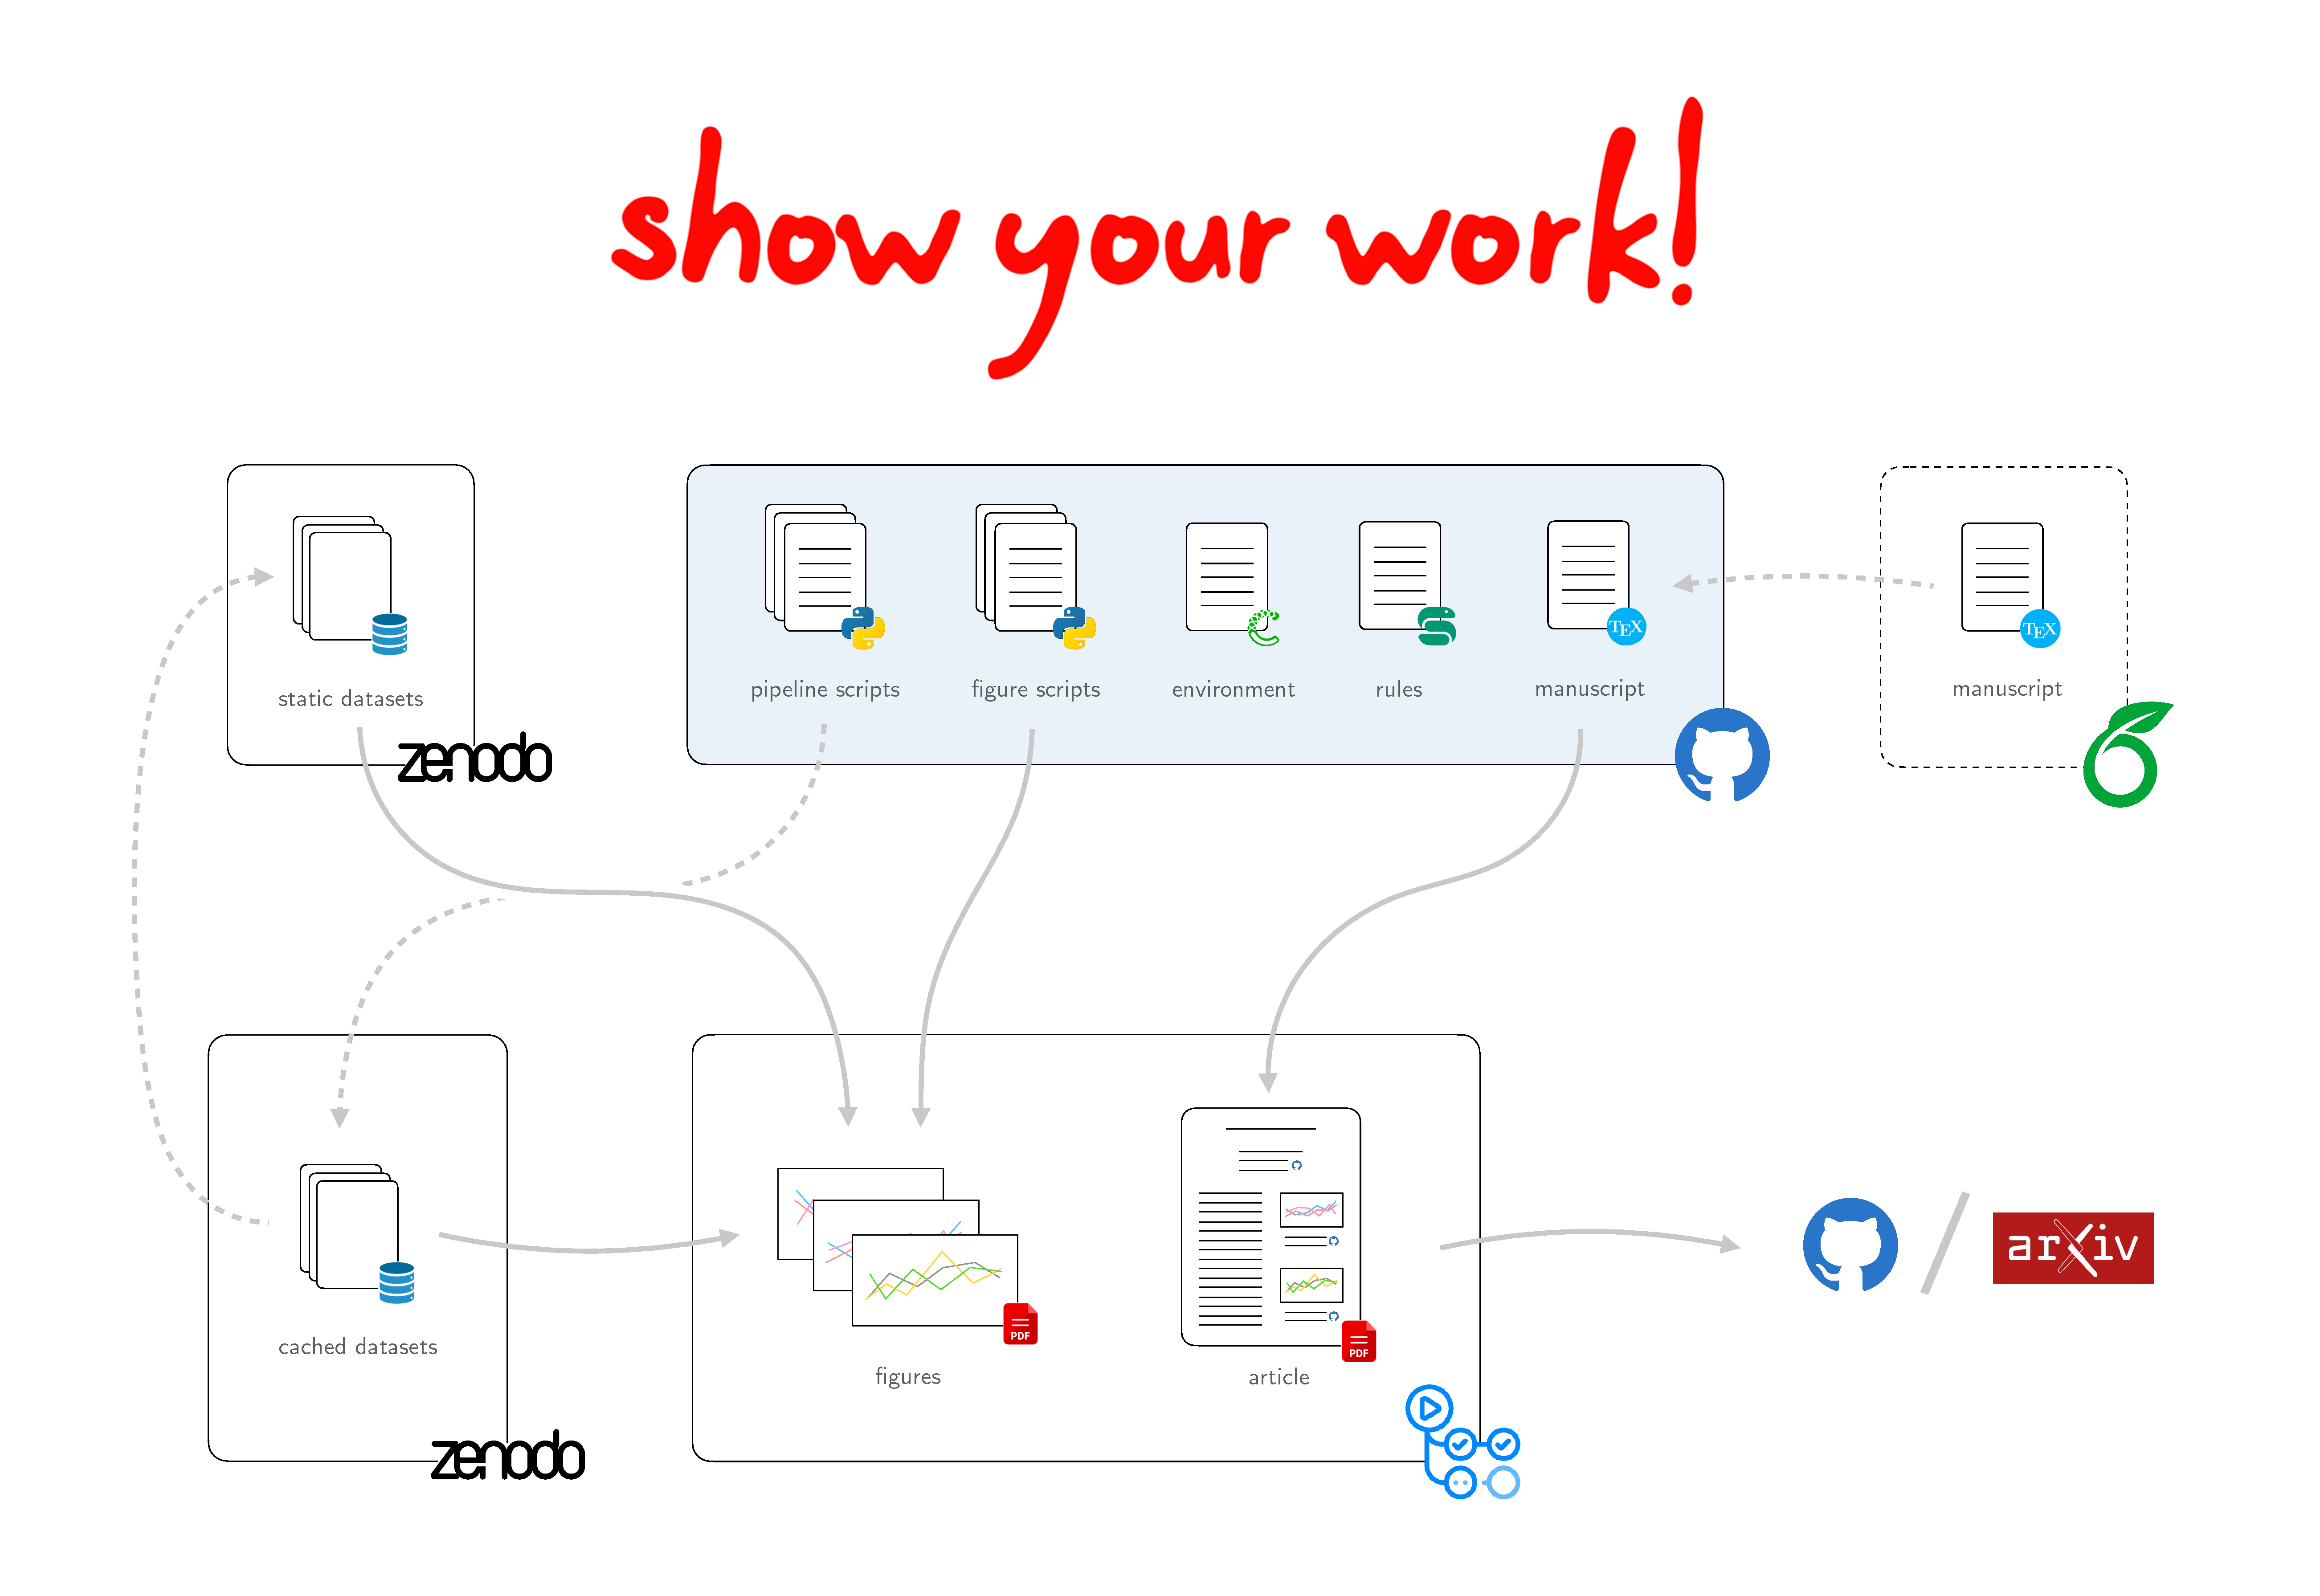
\includegraphics[width=\linewidth]{figures/overview.pdf}
        \caption{
            Overview of the \syw workflow for a scientific article.
            All code and instructions to compile the article exist within a \GitHub repository (top center), optionally synced with an \Overleaf project (top right).
            Upon every commit, a \GitHub Action is triggered to build the article in an isolated environment.
            Scripts are executed to generate figures and other workflow output (bottom center), optionally downloading version-controlled datasets from Zenodo (top left), and optionally caching intermediate results on Zenodo Sandbox (bottom left).
            Finally, the compiled article \pdf file, alongside an arXiv-compatible tarball, are generated and pushed to a special branch on the \GitHub repository.
        }
        \label{fig:overview}
    \end{centering}
\end{figure}

The ideas presented here are not new; nor are the ways in which they are implemented.
Instead, the main goal of \syw is to make developing---and using---reproducible scientific articles as easy as possible.
\syw works out of the box for simple projects, in which each figure in the article can be generated by running a given script. 
But it also works for more complicated pipelines, such as projects that depend on many intermediate steps or those that require running expensive simulations. 
The workflow interfaces directly with \Zenodo, allowing users to automatically upload the results of simulations so that expensive build steps can be bypassed on the cloud. 
In fact, most of the features under the hood are there to make the workflow as flexible and customizable as possible.

Papers that use \syw can be reproduced by downloading the associated repository and running the \syw command-line tool. 
Such papers (like this one!) include clickable icons next to each of their figures linking to (1) the exact version of the script used to generate them and (2) the exact version(s) of the dataset(s) used in their creation.

\section{Using {\protect\syw}}
\label{sec:usage}
In this section we provide basic, high-level instructions on how to install and use \syw.
These instructions are for version \VERSION of the code, the current version at the time of writing (\MONTHYEAR) and are subject to change in future releases.
For more details, including custom commands, settings, examples, and troubleshooting tips, please refer to the documentation for the specific version of \syw.

\subsection{Prerequisites}
\label{sec:usage:prereq}
\syw requires the \conda package manager and is currently tested only on Unix-like operating systems (such as Linux, Ubuntu, or MacOS).
Users must also have access to a \GitHub account; other \git platforms are not currently supported.
Note that users do \emph{not} need a local installation of a \TeX distribution, as \syw uses the \conda-managed \tectonic package to compile articles.

\subsection{Installation}
\label{sec:usage:install}
\syw can be installed with the \Python package manager \pip:\\

\noindent\begin{minipage}{\linewidth}
\begin{lstlisting}[
    style=bash
]
pip install -U showyourwork
\end{lstlisting}
\end{minipage}

\noindent (recommended) or from source on \GitHub:\\

\noindent\begin{minipage}{\linewidth}
\begin{lstlisting}[
    style=bash
]
git clone https://github.com/showyourwork/showyourwork
cd showyourwork
python setup.py install .
\end{lstlisting}
\end{minipage}

\subsection{Reproducing an article}
\label{sec:usage:reproduce}
Any project based on \syw can be reproduced by cloning its \GitHub repository and running \syw. For example, to reproduce the exact version of this paper that you are currently reading, run:\\

\noindent\begin{minipage}{\linewidth}
\begin{lstlisting}[
    style=bash,
    escapeinside={|}{|}
]
git clone https://github.com/showyourwork/showyourwork-paper
cd showyourwork-paper
git checkout |\GitHubSHA|
showyourwork
\end{lstlisting}
\end{minipage}

\noindent This will set up a custom \conda environment for the workflow, download the required datasets from \Zenodo, build all of the figures, and generate a \pdf file identical to this one.

\subsection{Creating a new article}
\label{sec:usage:new}
New projects may be created by running\\

\noindent\begin{minipage}{\linewidth}
\begin{lstlisting}[
    style=bash,
    otherkeywords={user,repo},
    emph={user,repo},
    emphstyle={\color{lsthilite}}
]
showyourwork setup user/repo
\end{lstlisting}
\end{minipage}



\noindent where \userarg and \repoarg are the user's \GitHub handle and the repository name, respectively. 
After the user answers a few prompts, \syw will set up a local \git repository \repoarg with the correct structure and placeholder files (see \S\ref{sec:usage:struct}).
The article may then be built by running\\

\noindent\begin{minipage}{\linewidth}
\begin{lstlisting}[
    style=bash
]
showyourwork
\end{lstlisting}
\end{minipage}

\noindent from the root of the repository.

\subsection{Repository structure}
\label{sec:usage:struct}
%
\begin{figure}[p!]
    \begin{centering}
        \includegraphics[width=0.5\linewidth]{figures/tree.pdf}
        \caption{
            The basic repository structure for an open source scientific article built with \syw.
            The article you are reading was generated from a repository with this exact structure; you can check it out \href{\commiturl}{here}.
            This figure was automatically generated from the \TikZ code in \repoargfile{src/scripts/tree.tex} by specifying a custom command in \repoargfile{showyourwork.yml}.
        }
        \label{fig:tree}
        \script{tree.tex}
    \end{centering}
\end{figure}
%
Figure~\ref{fig:tree} shows the basic directory structure for a \syw article repository as of version \VERSION{}.
Repositories are comprised of configuration files at the root level and a directory called \repoargfile{src} containing the manuscript files and all of the the code and workflow scripts needed to render the final article \pdf file.
%
\todo[rodluger]{More details here.}

\section{How it works}
\label{sec:how-it-works}
\todo[rodluger]{Discuss how things are actually implemented. Talk about the dependence on \snakemake \citep{Molder2021} and \tectonic. Discuss the integration with \Zenodo for both static datasets and cached datasets. Discuss integration with \Overleaf.}

\section{Examples}
\label{sec:examples}
In this section, we showcase a few projects based on \syw to illustrate how the workflow can facilitate the development and dissemination of open source scientific articles.

The most fundamental feature of \syw is the automatic generation of the figures in a paper, such as Figure~\ref{fig:eccentricity}, which we reproduce from \citet{Wagg2022}.
This figure was generated from the script \repoargfile{src/scripts/eccentricity.py} and has only a single other dependency: the \conda environment file \repoargfile{environment.yml} (see Figure~\ref{fig:dag}).

To establish dependencies between scripts and figures included in the TeX manuscript, users may provide the custom \scriptcmd command within the \figenv environment, where \scriptarg is the name of the script \syw should execute to generate the figure(s) within the current environment.
Additional dependencies may be specified explicitly in the \repoargfile{showyourwork.yml} configuration file or implicitly via custom rules in the \repoargfile{Snakefile}.

As a seconde example, consider Figure~\ref{fig:luhman16b}, which we reproduce from \citet{Luger2021c}. 
Unlike Figure~\ref{fig:eccentricity}, this figure has an external dependency: a Zenodo-hosted dataset containing the \emph{CRIRES} observations of the spectrum of a brown dwarf.
Users simply specify the DOI of the dataset and the files they wish to make dependencies of a given figure in \repoargfile{showyourwork.yml}, and \syw will download the data as needed.

Figure~\ref{fig:two_moons} is an example of a figure depending on an intermediate result that is cached on Zenodo Sandbox.
\todo[rodluger]{More details.}

\todo[rodluger]{Discuss Table~\ref{tab:variable} and variable output.}
Variable output can also occur inline. For instance, the following sentence is programmatically generated from the same script: 
\variable{output/kernel_value.tex}
Note the icon in the margin that automatically links to the corresponding \snakemake rule, where users can easily change the values of the kernel parameters.

\todo[rodluger]{Discuss Figure~\ref{fig:dag} and this paper as a whole as a meta-example.}

\todo[rodluger]{Finally, cite a bunch of papers here that already use showyourwork and showcase its various features.}

\section{Current issues and future work}
\label{sec:future}
\todo[rodluger][dfm][mathren][milescranmer]{This is a work in progress. Currently focused primarily on short-term reproducibility; discuss the various issues that arise from relying on \GitHub, \conda, \pip, etc. Broken links will be an issue. Conda environments are not impermeable. Currently difficult (impossible?) to run stuff on a cluster. Doesn't play nice with journals. Anything  else?}

\section{Conclusion}
\label{sec:conclusion}
\todo[rodluger][dfm][adrn][milescranmer][jfcrenshaw][mathren][katiebreivik][tomwagg]{Stuff here. showyourwork is a community project -- please contribute!}

% DEBUG -- place figures inline with text
\clearpage

\begin{figure}[p!]
    \begin{centering}
        \includegraphics[width=0.75\linewidth]{figures/eccentricity.pdf}
        \caption{
            The effect of binary eccentricity on the detectability of a \emph{LISA} gravitational wave source; reproduced from Figure 3 in \citet{Wagg2022}. 
            This figure was automatically generated from the script \repoargfile{src/scripts/eccentricity.py}.
            The \GitHub icon in the margin is a clickable link pointing to the exact version of the script on \GitHub used to produce this figure.
        }
        \label{fig:eccentricity}
        \script{eccentricity.py}
    \end{centering}
\end{figure}

\begin{figure}[p!]
    \begin{centering}
        \includegraphics[width=0.75\linewidth]{figures/luhman16b.pdf}
        \caption{
            16 \emph{CRIRES} spectra of WISE 1049-5319B spanning a full rotation period of the brown dwarf; adapted from Figure 14 in \citet{Luger2021c} and based on data from \citet{Crossfield2014}.
            This figure was automatically generated from the script \repoargfile{src/scripts/luhman16b.py} and a dataset downloaded from \Zenodo.
            In addition to the \GitHub icon linking to the script, this figure also has a dataset icon linking to the Zenodo deposit that hosts the data needed to generate it.
        }
        \label{fig:luhman16b}
        \script{luhman16b.py}
    \end{centering}
\end{figure}

\begin{figure}[p!]
    \begin{centering}
        \includegraphics[width=0.75\linewidth]{figures/two_moons.pdf}
        \caption{
            A normalizing flow demonstrated on the two moons data set from \scikitlearn;
            reproduced from Figure 1 in \citet{Crenshaw2022}.
            This figure was automatically generated from the script \repoargfile{src/scripts/two\_moons.py}
            and an intermediate dataset that was automatically cached on \Zenodo.
        }
        \label{fig:two_moons}
        \script{two_moons.py}
    \end{centering}
\end{figure}

\begin{table}
    \begin{center}
        \begin{tabular}{@{}l|l@{}}
            \hline
            Name & Representation \\
            \hline
            \variable{output/kernels.tex}
        \end{tabular}
    \end{center}
        \caption{The functional forms of various commonly used Gaussian process kernels; based on Table~1 in \citet{Aigrain2022}.
        The contents of this table are programmatically generated; the kernels are defined as \sympy expressions and rendered into \TeX form in the script \repoargfile{src/scripts/kernels.py}.
        The autogenerated \GitHub icon in the margin links to the rule in the \repoargfile{Snakefile} that runs that script.
    }
    \label{tab:variable}
\end{table}

\begin{sidewaysfigure}
    \begin{centering}
        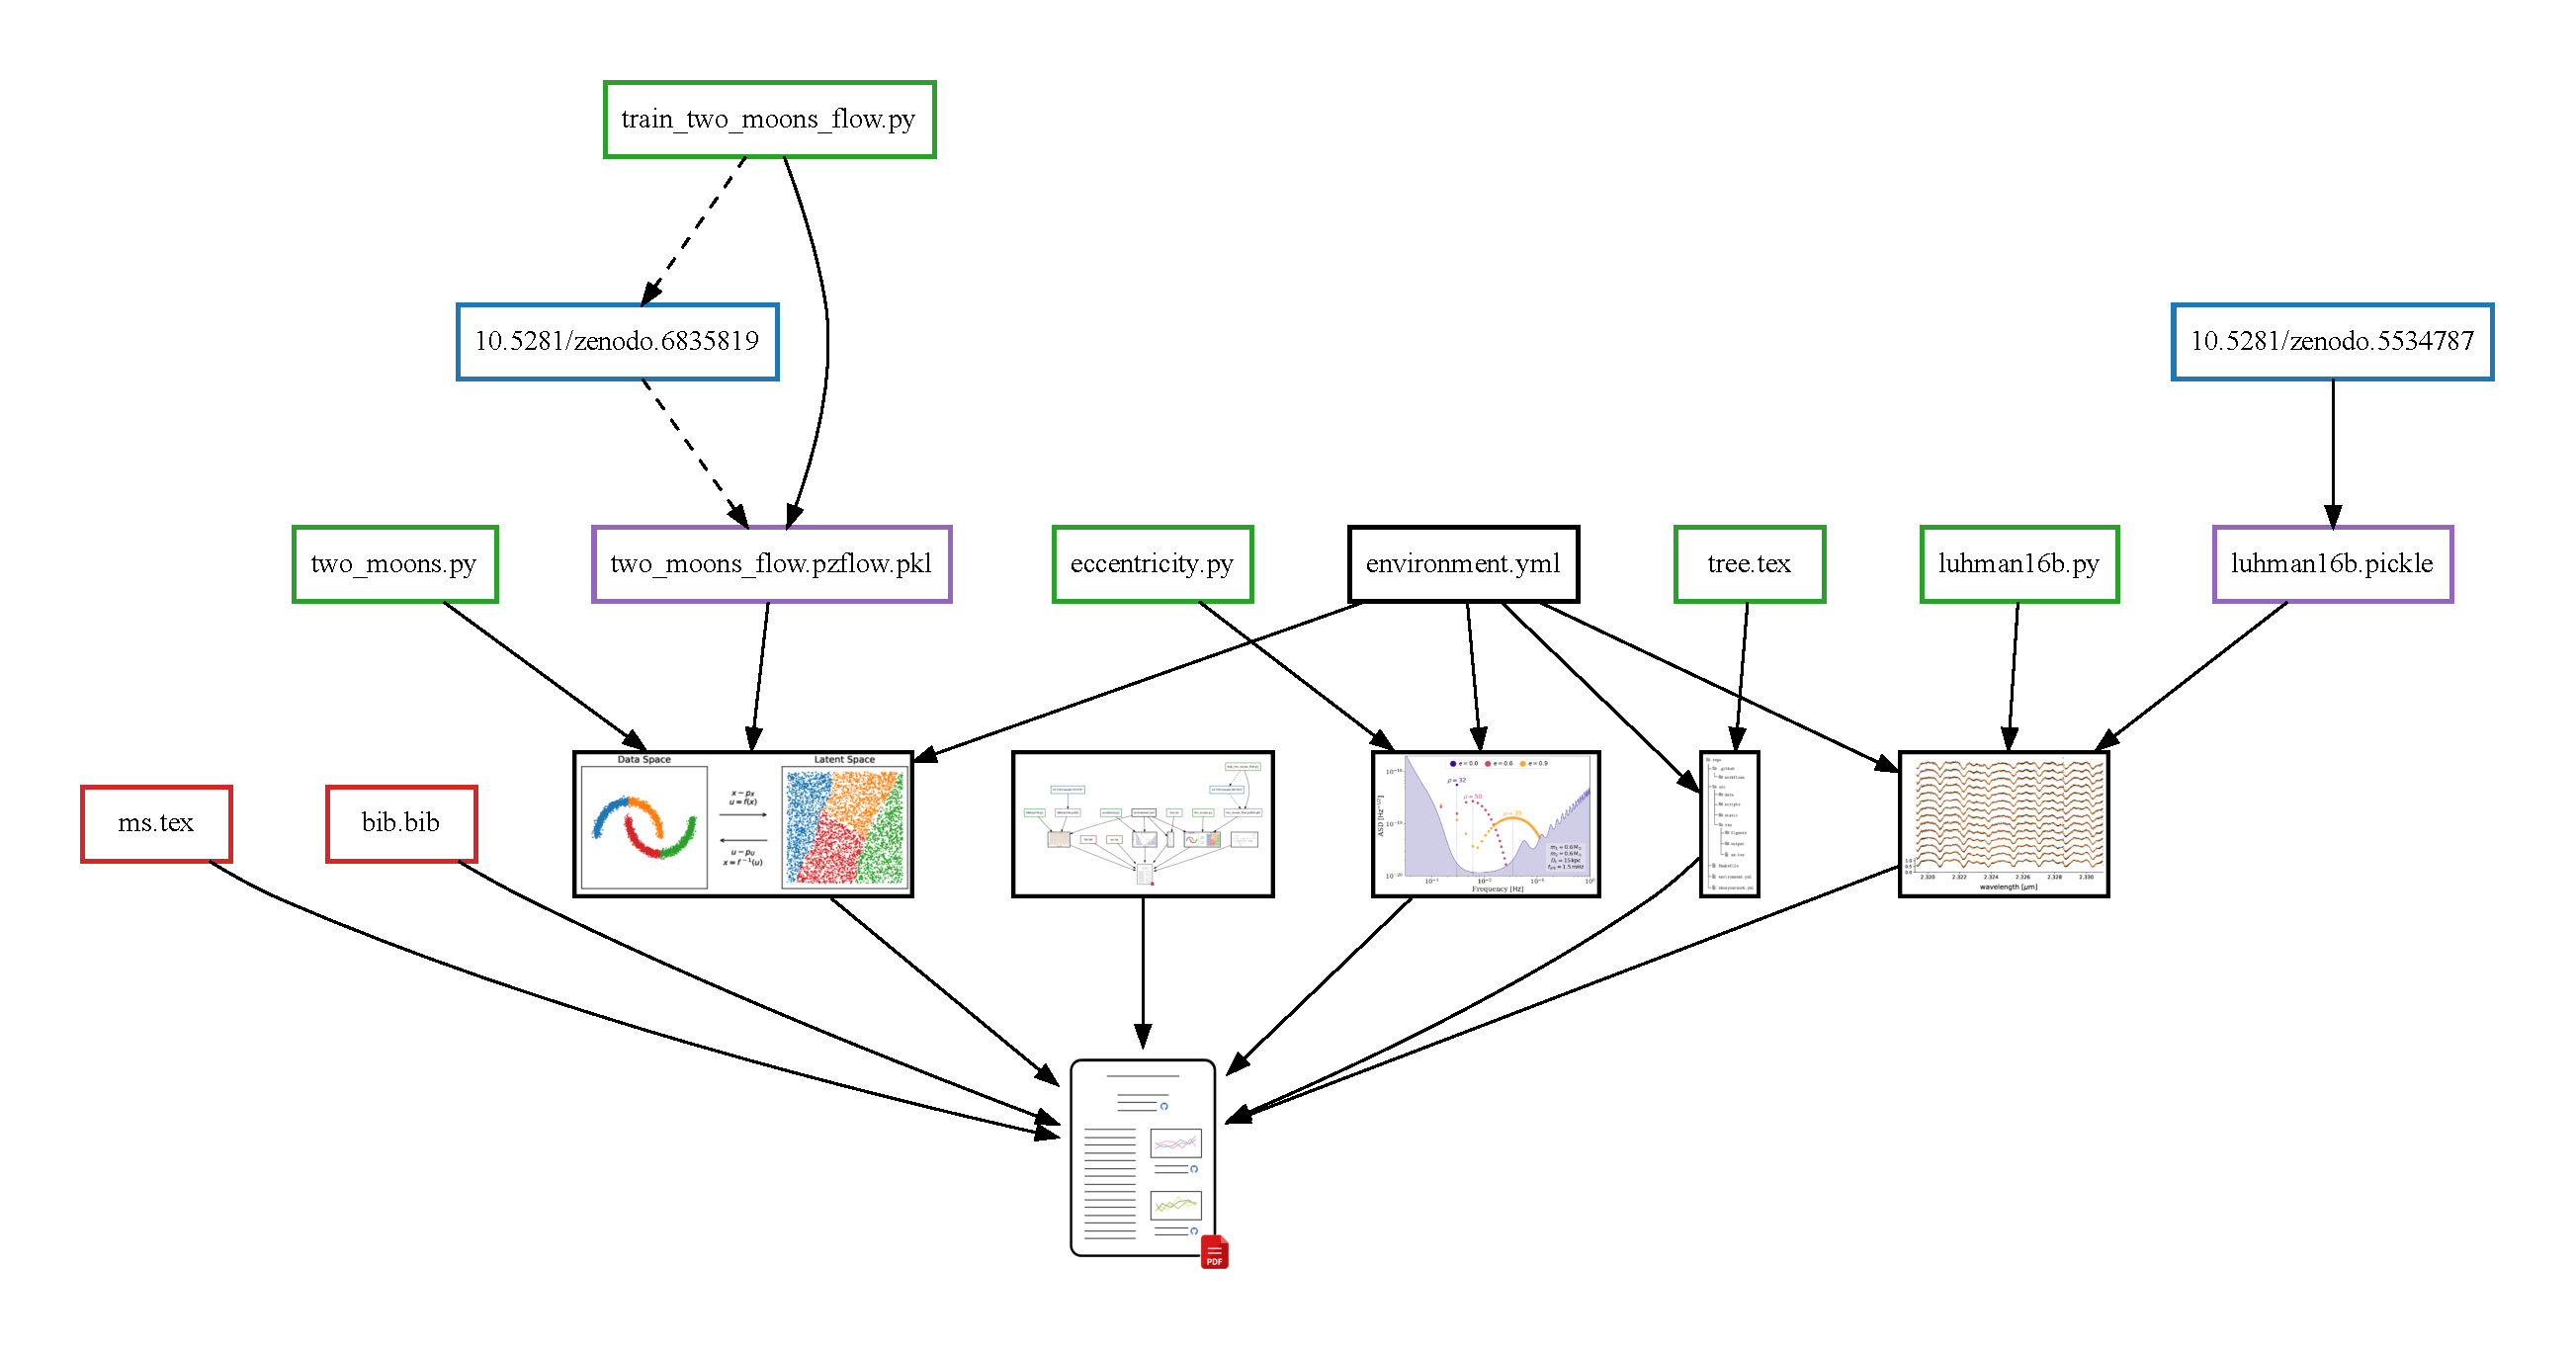
\includegraphics[width=\linewidth]{figures/dag.pdf}
        \caption{
            A directed acyclic graph (DAG) showing the complete list of dependencies for the article. 
            Scripts are shown in green, \Zenodo deposits in blue, datasets in purple, and \TeX files in red.
            This figure is located in the \repoargfile{src/static} directory and, unlike the other figures in this article, is version controlled by \git. The \repoargfile{src/static} directory is reserved for figures that are not programmatically generated and simply get copied over to the output directory at compile time.
        }
        \label{fig:dag}
    \end{centering}
\end{sidewaysfigure}

\bibliography{bib}

\end{document}